\documentclass[11pt]{article}

% Packages
\usepackage[utf8]{inputenc}
\usepackage[T1]{fontenc}
\usepackage{times}
\usepackage[margin=0.85in]{geometry}
\usepackage{graphicx}
\usepackage{booktabs}
\usepackage{amsmath}
\usepackage{amssymb}
\usepackage{hyperref}
\usepackage{microtype}
\usepackage{multirow}
\usepackage{caption}
\usepackage{subcaption}
\usepackage{natbib}
\usepackage{xcolor}
\usepackage{enumitem}
\usepackage{float}
\usepackage{array}
\usepackage{multicol}
\usepackage{colortbl}
\usepackage{titlesec}

% Tighter section spacing
\titlespacing*{\section}{0pt}{10pt}{5pt}
\titlespacing*{\subsection}{0pt}{8pt}{4pt}
\titlespacing*{\paragraph}{0pt}{6pt}{4pt}

% Hyperref setup
\hypersetup{
    colorlinks=true,
    linkcolor=blue!70!black,
    citecolor=green!50!black,
    urlcolor=blue!70!black
}

% Define colors
\definecolor{headerblue}{RGB}{41,128,185}
\definecolor{lightblue}{RGB}{214,234,248}
\definecolor{lightgreen}{RGB}{212,239,223}
\definecolor{lightred}{RGB}{250,219,216}
\definecolor{lightyellow}{RGB}{254,249,231}
\definecolor{darkgreen}{RGB}{39,174,96}
\definecolor{darkred}{RGB}{192,57,43}
\definecolor{ourscolor}{RGB}{39,174,96}

% Custom commands
\newcommand{\fone}{F\textsubscript{1}}
\newcommand{\method}{Active GLiNER}

% Title
\title{\LARGE\textbf{Active GLiNER: Efficient Named Entity Recognition\\[4pt]
Through LoRA Fine-Tuning, Uncertainty-Based Data Selection,\\[4pt]
and Synthetic Label Mixing}}

\author{
    \large Abhishek Thomas \\[2pt]
    \normalsize\textit{emlyon business school} \\
    \normalsize\textit{MSc Data Science \& AI Strategy} \\[2pt]
    \normalsize\texttt{abhishek01789@gmail.com}
}

\date{}

\begin{document}
\maketitle

% ============================================================
% ABSTRACT
% ============================================================
\begin{abstract}
\noindent Named Entity Recognition (NER) systems in production face a difficult choice between the accuracy of large language models (LLMs) and the efficiency of lightweight models. We present \method{}, a framework that bridges this gap by combining GLiNER, a span-based NER architecture, with Low-Rank Adaptation (LoRA), uncertainty-based data selection, and strategic mixing of human and LLM-generated labels. On the MIT Movies dataset, LoRA fine-tuning with only 4\% of trainable parameters achieves 88.5 \fone{}, matching full fine-tuning and substantially outperforming both the zero-shot baseline (46.6 \fone{}) and a Gemma 3 12B teacher model (69.7 \fone{}). We compare four acquisition functions for selecting informative training examples and find that simple minimum confidence is the most effective strategy for span-based models, reaching 80 \fone{} with just 200 labeled sentences. We further show that replacing up to 25\% of human annotations with LLM-generated labels maintains performance within one \fone{} point of full supervision. These results demonstrate that carefully configured lightweight models can achieve near-LLM accuracy at less than 1\% of the operational cost. Code is available at \url{https://github.com/dcrey7/active_gliner}.
\end{abstract}

\vspace{4pt}

\begin{multicols}{2}

% ============================================================
% 1. INTRODUCTION
% ============================================================
\section{Introduction}

Named Entity Recognition (NER) is a core component of information extraction systems, supporting applications from document analysis to knowledge graph construction \citep{keraghel2024survey}. While large language models such as GPT-4 and Gemini achieve strong NER performance through prompting, their deployment in production introduces substantial challenges: high inference costs, latency, rate limits, lack of fine-tuning access, and data privacy concerns \citep{belcak2025small}.

These limitations have motivated a growing interest in lightweight, specialized models that can be deployed on premises with predictable costs. GLiNER \citep{zaratiana2023gliner} represents a promising direction in this space. Unlike traditional sequence taggers, GLiNER formulates NER as a span classification problem, directly scoring candidate entity spans against natural language type descriptions. This design enables zero-shot recognition of arbitrary entity types while maintaining the efficiency of a BERT-scale encoder.

However, adapting GLiNER to specific domains requires labeled data, and obtaining high quality annotations is expensive. Two complementary strategies can reduce this cost: (1) \emph{uncertainty-based data selection}, where the model identifies the most informative examples for annotation, and (2) \emph{synthetic label generation}, where an LLM provides annotations for a portion of the training data. The question is whether these strategies, combined with parameter-efficient fine-tuning, can produce a system that is competitive with direct LLM inference at a fraction of the cost.

We present \method{}, a framework that integrates these three components into a single pipeline. Our contributions are:

\begin{enumerate}[leftmargin=*, nosep, itemsep=2pt]
    \item We show that LoRA fine-tuning of GLiNER matches full fine-tuning (88.5 \fone{}) while updating only 4\% of parameters, and identify the optimal layer configuration through systematic ablation.
    \item We adapt four uncertainty-based acquisition functions to GLiNER's span-based architecture, finding that minimum confidence is the most robust choice for data selection.
    \item We conduct a systematic study of mixing human and LLM-generated labels, showing that 75\% human with 25\% synthetic labels performs within one \fone{} point of full supervision.
    \item We provide a cost analysis showing over 99\% reduction in operational NER costs compared to continuous LLM inference.
\end{enumerate}

% ============================================================
% 2. RELATED WORK
% ============================================================
\section{Related Work}

\paragraph{GLiNER and Span-Based NER.}
GLiNER \citep{zaratiana2023gliner} introduced a span-based approach to NER that processes entity type descriptions alongside input text through a shared bidirectional encoder. The architecture has since expanded to GLiNER-multitask \citep{stepanov2024glinermultitask}, GLiNER2 \citep{zaratiana2025gliner2}, and the bi-encoder variant \citep{stepanov2026gliner_bi} which decouples text and label encoding for scalability to thousands of entity types. Our work focuses on domain adaptation of the bi-encoder architecture through parameter-efficient fine-tuning.

\paragraph{Parameter-Efficient Fine-Tuning.}
LoRA \citep{hu2021lora} reduces fine-tuning cost by introducing small trainable matrices into frozen pretrained weights. While widely adopted for generation tasks, its application to span-based NER models remains underexplored. The GLiNER architecture exposes multiple candidate module groups for adaptation. We present the first systematic study of LoRA layer selection for GLiNER.

\paragraph{Active Learning for NER.}
Active learning reduces annotation cost by prioritizing informative examples. \citet{shen2017deep} introduced MNLP for NER, and \citet{siddhant2018deep} showed that Bayesian uncertainty estimates improve sample efficiency. However, all prior NER active learning work targets sequence taggers with token-level BIO tags. GLiNER's span-based predictions yield per-entity confidence scores, requiring different aggregation strategies. Our setup follows a single-round selection protocol (simulated active learning), ranking all examples by uncertainty without iterative re-ranking \citep{lowell2019practical}.

\paragraph{LLM-Generated Labels for NER.}
UniversalNER \citep{zhou2024universalner} showed that distilling LLM annotations into smaller models can match the teacher's performance. ProgGen \citep{heng2024proggen} and GuideX \citep{fuente2025guidex} generate synthetic NER data through structured prompting. \citet{kamath2025synthetic} found that even 100 human-annotated examples outperform larger amounts of purely synthetic data. Unlike these approaches, we study the \emph{mixing ratio} between human and synthetic labels within a fixed budget.

% ============================================================
% 3. METHOD
% ============================================================
\section{Method}

\subsection{Framework Overview}

The \method{} framework consists of four stages: (1) establish zero-shot baselines for GLiNER and an LLM teacher, (2) rank training examples by uncertainty using span-level confidence scores, (3) fine-tune GLiNER with LoRA on subsets of the most uncertain examples using human labels, LLM labels, or mixtures, and (4) evaluate on a held-out test set using span-level metrics and confidence analysis.

\subsection{Model Architecture}

We use the GLiNER bi-encoder large model (v1.0) published by Knowledgator.\footnote{\url{https://huggingface.co/knowledgator/modern-gliner-bi-large-v1.0}} It is built on ModernBERT-large with BGE-base-en-v1.5 as the label encoder. The model scores all candidate spans against entity type descriptions and produces per-span confidence scores between 0 and 1. It supports contexts up to 8{,}192 tokens.

\subsection{LoRA Configuration}

LoRA adapters are applied to selected layers. We test eight configurations across four module groups: \textbf{ModernBERT} (Wqkv, Wo, Wi, projection), \textbf{BERT-style} (query, key, value, dense layers), \textbf{Attention} (combined attention modules), and \textbf{Task-specific} (span and prompt representation layers). Hyperparameters are tuned with Optuna \citep{akiba2019optuna}. The final configuration uses rank 16, alpha 32, dropout 0.1, batch size 12, and 2{,}500 training steps with early stopping.

\subsection{Acquisition Functions}

For each sentence, we aggregate span confidence scores into a single uncertainty value:

\begin{itemize}[leftmargin=*, nosep, itemsep=2pt]
    \item \textbf{Minimum Confidence (LC)}: Lowest span score.
    \item \textbf{MNLP}: Average negative log confidence across spans, adapted from \citet{shen2017deep}.
    \item \textbf{MSE}: Mean of $(1 - c_i)^2$ across spans, giving stronger weight to low-confidence predictions.
    \item \textbf{Random}: Baseline with no uncertainty signal.
\end{itemize}

Sentences with no predicted or ground truth entities are excluded from ranking.

\subsection{Synthetic Label Generation}

We use Gemma 3 12B (local, via Ollama) as the label generator. Each sentence receives a prompt listing the 12 entity types with instructions to return a JSON object. Responses pass through validation: JSON parsing, schema checking, entity text verification against the source sentence, type filtering, and conversion to token-level spans.

\subsection{Training Data Composition}

For mixing experiments, training sets of size $N$ are drawn from the uncertainty-ranked pool. A fraction $r$ of sentences use human labels, the rest use LLM labels. We test $r \in \{0, 0.25, 0.50, 0.75, 1.0\}$ to simulate varying annotation budgets.

\end{multicols}

% ============================================================
% FRAMEWORK FIGURE (full width)
% ============================================================
\begin{figure*}[t]
    \centering
    \fcolorbox{headerblue}{white}{%
    \begin{minipage}{0.95\textwidth}
    \vspace{8pt}
    \centering
    {\large\bfseries Active GLiNER Framework}\\[10pt]
    %
    % Row 1: Main pipeline boxes
    \resizebox{0.93\textwidth}{!}{%
    \begin{tabular}{ccccccccc}
    \fcolorbox{headerblue}{lightblue!50}{\parbox{2.0cm}{\centering\small\textbf{Input Data}\\[2pt]\scriptsize MIT Movies\\9,774 sentences}}
    & {\Large$\boldsymbol{\rightarrow}$} &
    \fcolorbox{headerblue}{lightyellow}{\parbox{2.2cm}{\centering\small\textbf{Zero-Shot\\Evaluation}\\[2pt]\scriptsize GLiNER Base\\+ LLM Baseline}}
    & {\Large$\boldsymbol{\rightarrow}$} &
    \fcolorbox{headerblue}{lightyellow}{\parbox{2.2cm}{\centering\small\textbf{Uncertainty\\Ranking}\\[2pt]\scriptsize LC / MNLP\\MSE / Random}}
    & {\Large$\boldsymbol{\rightarrow}$} &
    \fcolorbox{darkred}{lightred}{\parbox{2.2cm}{\centering\small\textbf{LoRA\\Fine-Tuning}\\[2pt]\scriptsize GT / LLM\\Mixed Labels}}
    & {\Large$\boldsymbol{\rightarrow}$} &
    \fcolorbox{darkgreen}{lightgreen}{\parbox{2.0cm}{\centering\small\textbf{Evaluation}\\[2pt]\scriptsize Span-level\\P / R / \fone{}}}
    \end{tabular}}
    \vspace{8pt}
    \end{minipage}}
    \caption{Overview of the Active GLiNER framework. Training examples are ranked by model uncertainty, then used for LoRA fine-tuning with human, LLM, or mixed labels. Evaluation uses human-annotated test data.}
    \label{fig:framework}
\end{figure*}

\begin{multicols}{2}

% ============================================================
% 4. EXPERIMENTAL SETUP
% ============================================================
\section{Experimental Setup}

\paragraph{Dataset.}
We evaluate on the MIT Movies dataset \citep{liu2019movie}, a slot-filling benchmark with natural language queries about films. The training split has 9{,}774 sentences with 21{,}294 entity mentions across 12 types. The test split has 2{,}442 sentences with 5{,}338 mentions. Genre (20.4\%) and actor (15.1\%) are the most frequent types; trailer (0.5\%) and song (1.2\%) the rarest.

\paragraph{Baselines.}
We compare: (1) GLiNER zero-shot, (2) GLiNER full fine-tuning (all parameters), and (3) Gemma 3 12B served locally via Ollama. As an additional reference, we also evaluated Qwen3 235B A22B through the Cerebras inference platform, which achieved approximately 75\% \fone{} on the test set, confirming that larger LLMs produce stronger but costlier baselines.

\paragraph{Evaluation.}
All models are evaluated using span-level micro-averaged \fone{}, precision, and recall. An entity is correct only if both span boundaries and type match exactly.

\paragraph{Implementation.}
Experiments run in Docker on two NVIDIA RTX 3090 GPUs with 48GB RAM. The modular codebase separates data loading, training, LLM interaction, and evaluation.

% ============================================================
% 5. RESULTS
% ============================================================
\section{Results}

\subsection{Baseline and Threshold Analysis}

Table~\ref{tab:baseline} presents the baseline results. GLiNER zero-shot achieves 46.6 \fone{}, while LoRA fine-tuning raises this to 85.4 \fone{} with only 4\% of parameters updated. Full fine-tuning reaches 87.0 \fone{}, confirming that LoRA captures most of the available gain. Gemma 3 12B achieves 57.2 \fone{} as a direct NER system.

\end{multicols}

% Baseline table (full width, colored)
\begin{table}[H]
    \centering
    \small
    \begin{tabular}{l c c c}
        \toprule
        \rowcolor{headerblue!15}
        \textbf{Configuration} & \textbf{Precision} & \textbf{Recall} & \textbf{\fone{}} \\
        \midrule
        GLiNER zero-shot (threshold=0.5) & 54.93 & 40.46 & 46.60 \\
        GLiNER + LoRA, full data (threshold=0.5) & 83.46 & 87.65 & \textbf{85.51} \\
        GLiNER full fine-tune & 80.2 & 89.1 & 87.0 \\
        \rowcolor{lightred!40}
        Gemma 3 12B (zero-shot) & 68.87 & 70.02 & 69.44 \\
        \bottomrule
    \end{tabular}
    \caption{Baseline performance on MIT Movies test set. LoRA fine-tuning nearly matches full fine-tuning while updating only 4\% of parameters.}
    \label{tab:baseline}
\end{table}

% Threshold figure (full width)
\begin{figure*}[t]
    \centering
    \begin{subfigure}[t]{0.32\textwidth}
        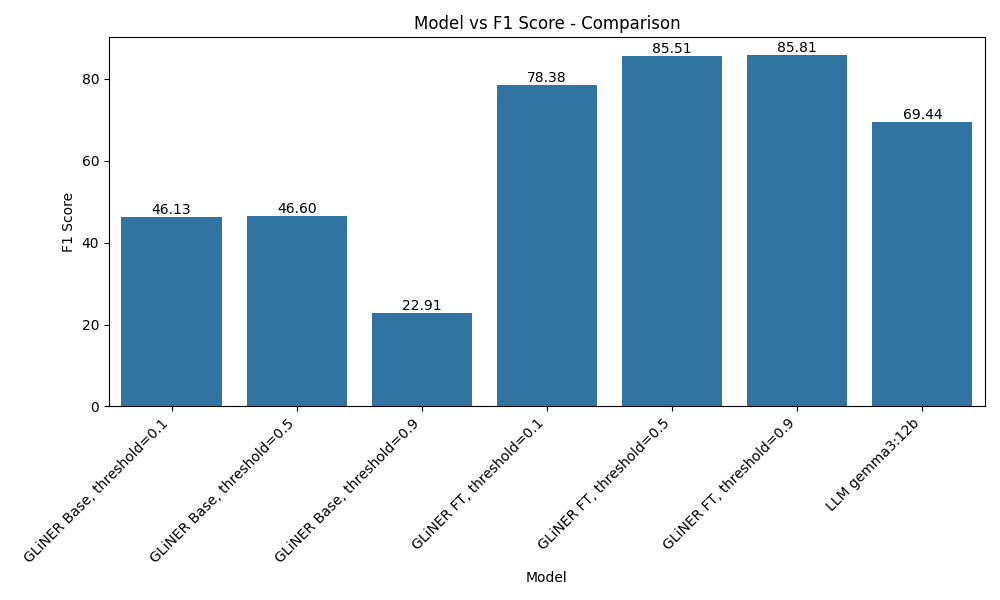
\includegraphics[width=\textwidth]{figures/threshold_f1.png}
        \caption{\fone{} comparison}
    \end{subfigure}
    \hfill
    \begin{subfigure}[t]{0.32\textwidth}
        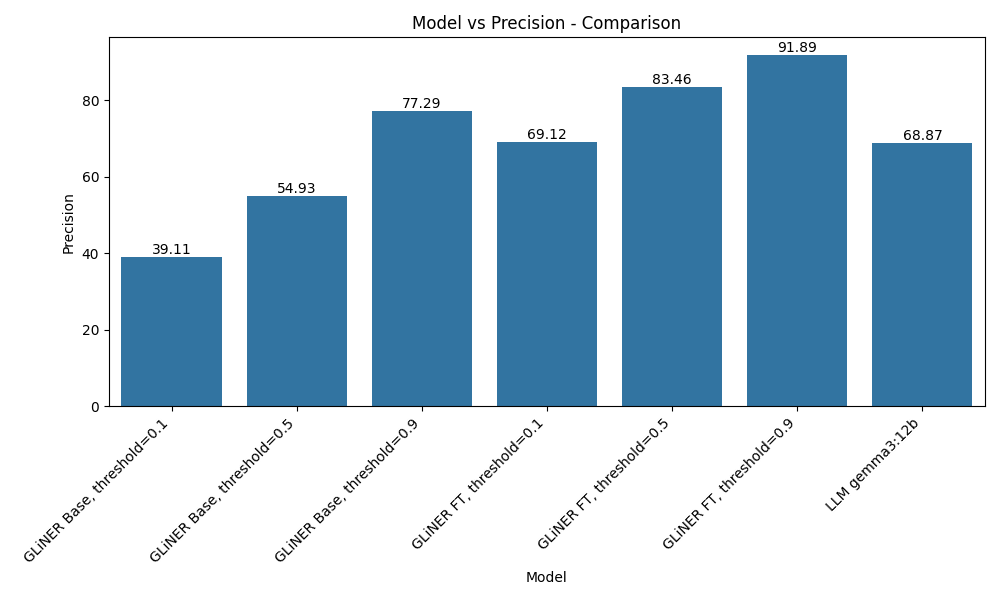
\includegraphics[width=\textwidth]{figures/threshold_precision.png}
        \caption{Precision comparison}
    \end{subfigure}
    \hfill
    \begin{subfigure}[t]{0.32\textwidth}
        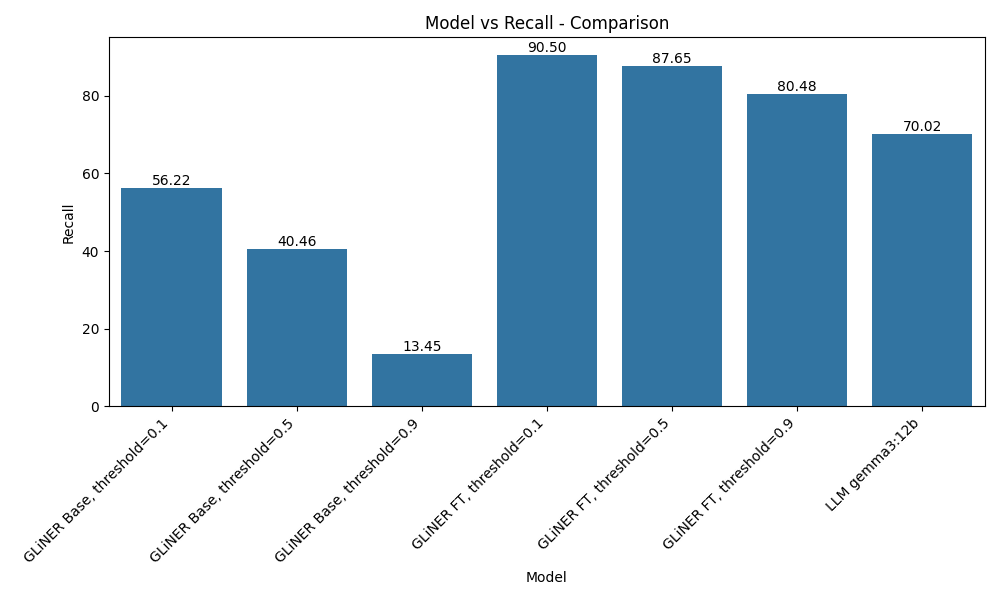
\includegraphics[width=\textwidth]{figures/threshold_recall.png}
        \caption{Recall comparison}
    \end{subfigure}
    \caption{Threshold analysis on MIT Movies test set. GLiNER Base and Fine-Tuned (FT) models are evaluated at confidence thresholds 0.1, 0.5, and 0.9, compared against the LLM baseline (Gemma 3 12B). Fine-tuned GLiNER at threshold 0.5 achieves the best balance of precision and recall, outperforming the LLM on \fone{}.}
    \label{fig:threshold}
\end{figure*}

\begin{multicols}{2}

Figure~\ref{fig:threshold} shows how confidence thresholds affect GLiNER's behavior. The zero-shot model is overconfident: threshold 0.1 and 0.5 yield similar \fone{} (${\sim}$46\%). After fine-tuning, threshold 0.5 delivers 85.5 \fone{} with balanced precision (83.5\%) and recall (87.7\%). The fine-tuned model at threshold 0.9 achieves 91.9\% precision but sacrifices recall to 80.5\%.

\subsection{LoRA Layer Selection}

Figure~\ref{fig:lora_layers} presents the layer selection study. ModernBERT + Task layers achieve the best \fone{} (88.76\%) with only 12 target modules. The top five configurations all include ModernBERT backbone layers and perform within 0.4 points of each other. In contrast, BERT-only (75.76\%) and task-only (67.73\%) configurations underperform sharply, confirming that both the encoder backbone and the task-specific heads must be adapted together.

\end{multicols}

% LoRA layers figure (full width)
\begin{figure*}[t]
    \centering
    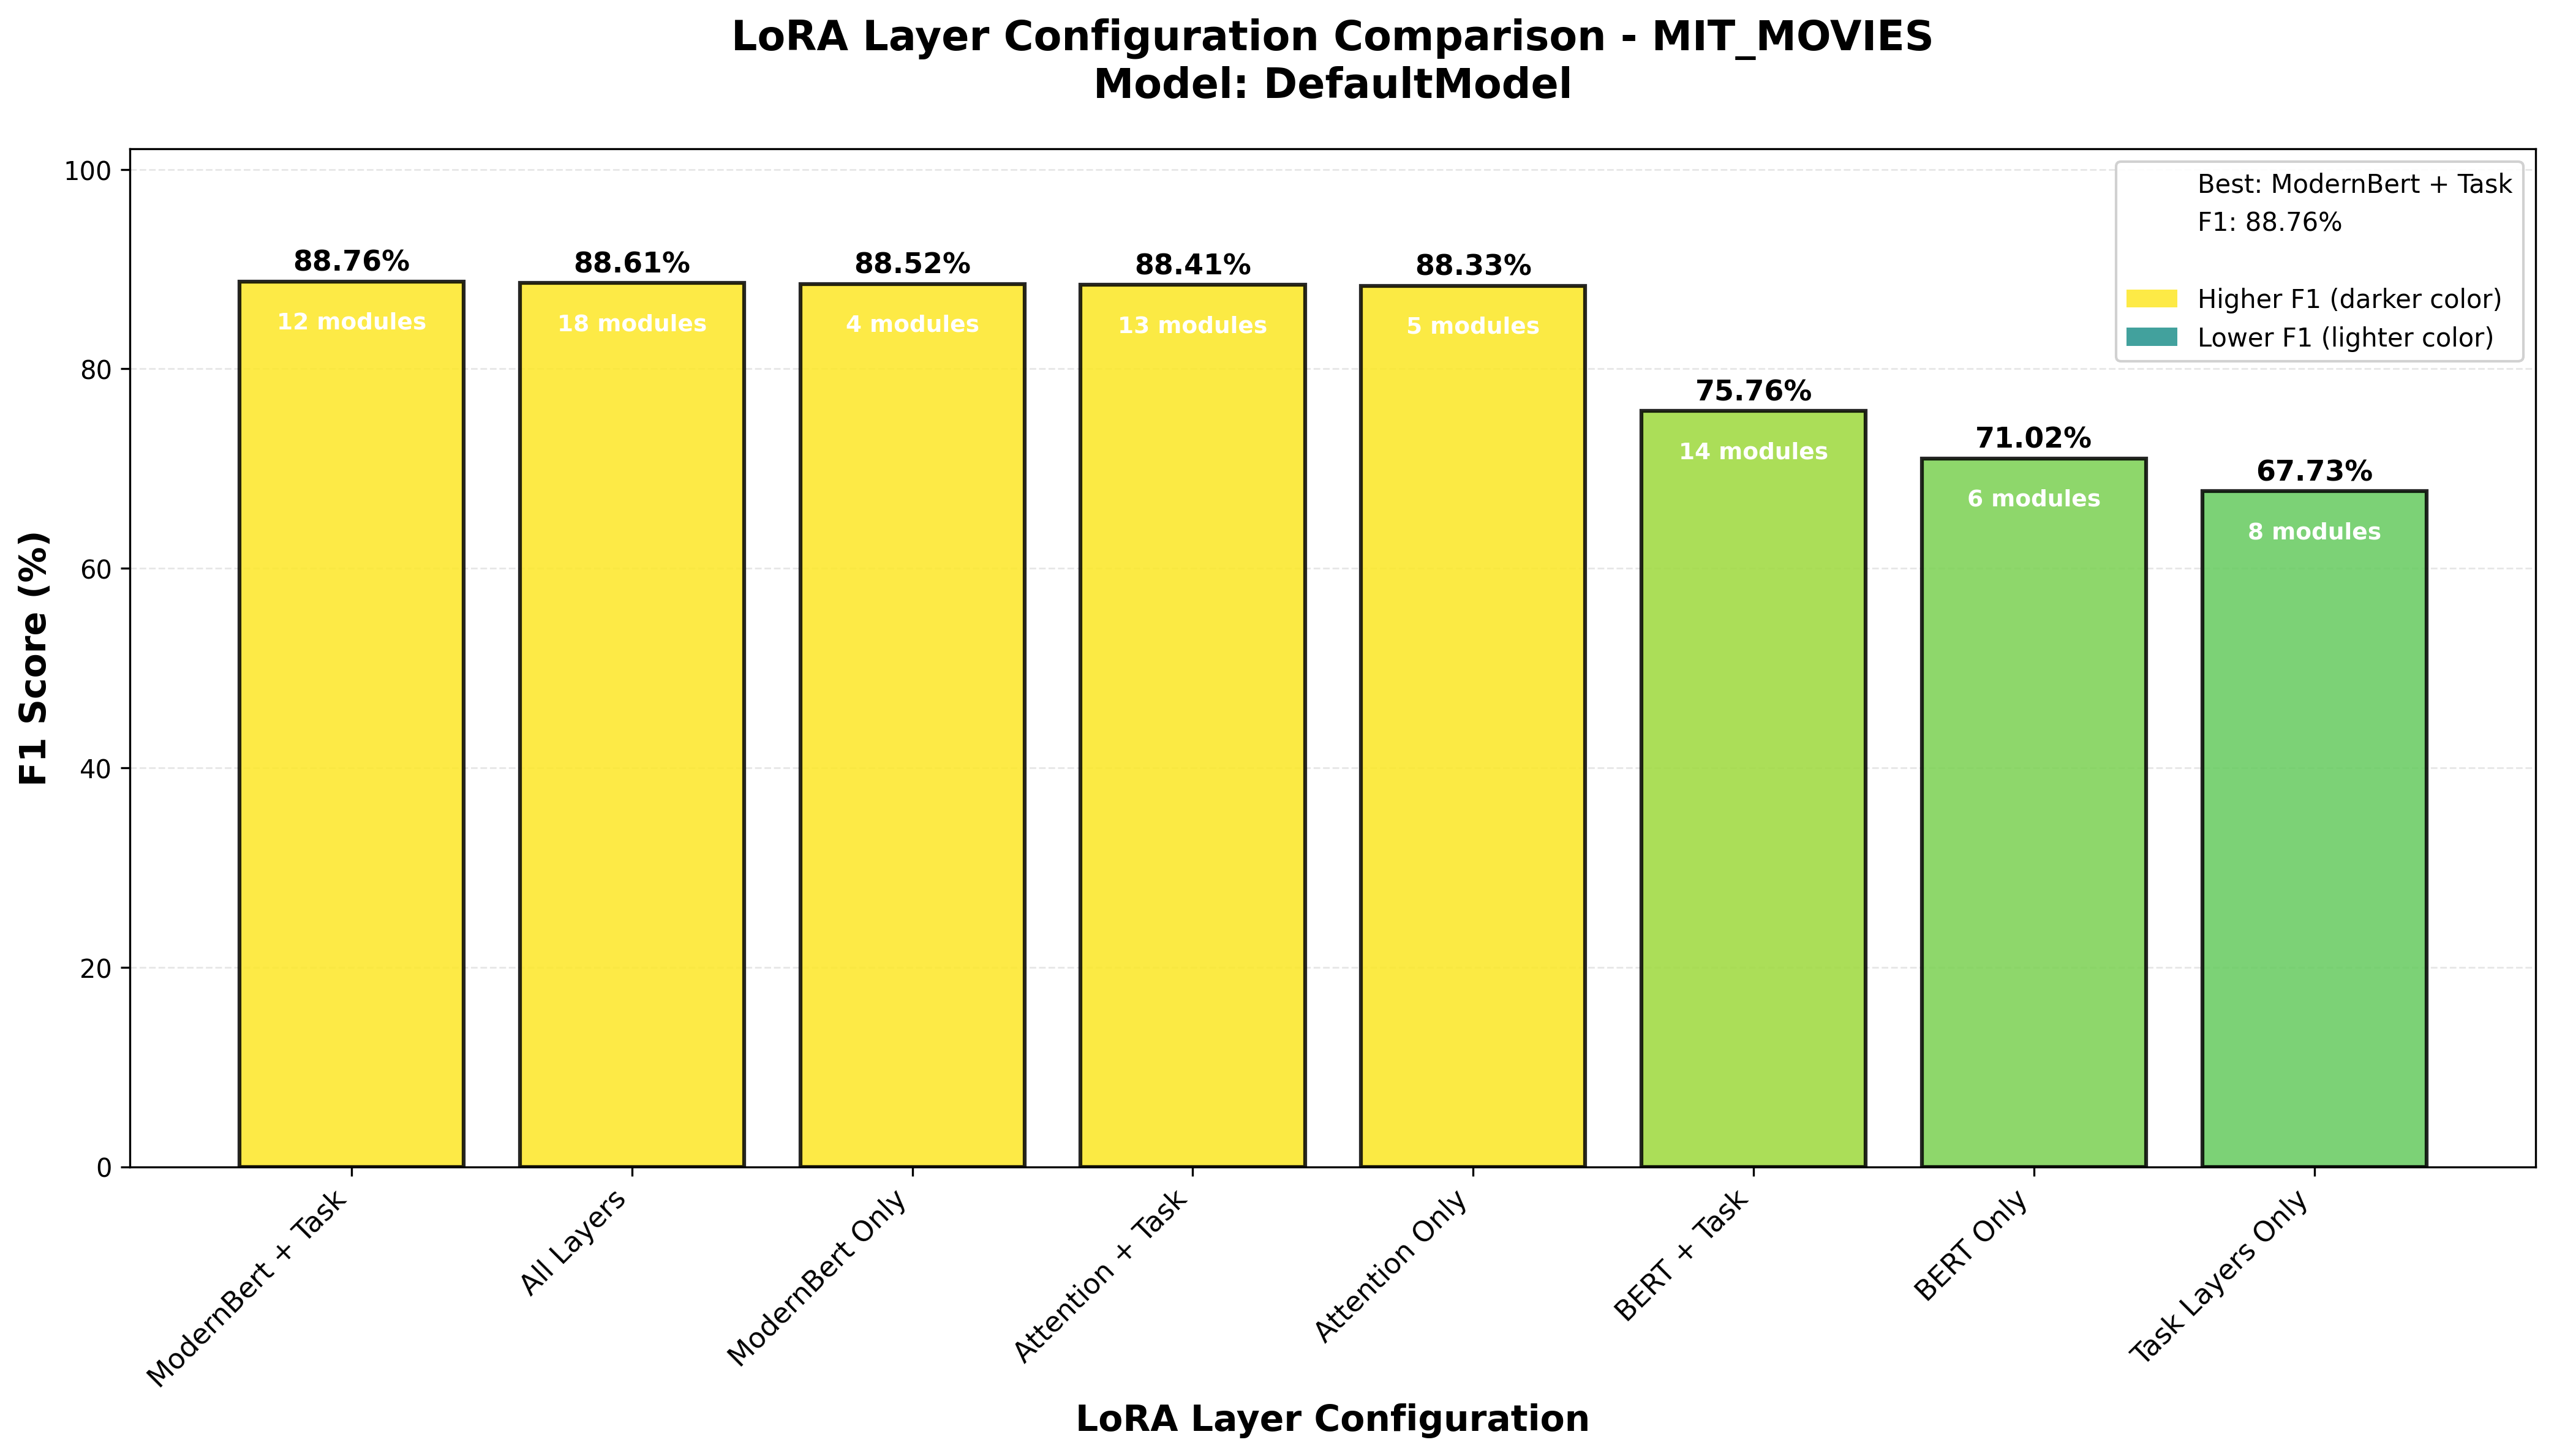
\includegraphics[width=0.85\textwidth]{figures/lora_layers.png}
    \caption{LoRA layer configuration comparison. Each bar shows the \fone{} achieved with different groups of target modules. The number of modules is annotated inside each bar. Configurations including ModernBERT layers (yellow) consistently outperform those without (green). The best configuration (ModernBERT + Task) uses only 12 modules.}
    \label{fig:lora_layers}
\end{figure*}

\begin{multicols}{2}

\subsection{Acquisition Function Comparison}

Table~\ref{tab:active_learning} and Figure~\ref{fig:active_learning} show how different acquisition strategies affect data efficiency. At small budgets (50 to 200 sentences), minimum confidence (LC) reaches 80 \fone{} first at just 200 examples. MNLP and MSE need about 400 examples to cross the same threshold. In the mid-budget range (400 to 1{,}500), all confidence-based strategies outperform random selection by 1 to 2 \fone{} points. At 2{,}500 sentences, the strategies converge, with LC ending at 86.02 \fone{}.

\end{multicols}

% Active learning table (full width, colored)
\begin{table}[H]
    \centering
    \small
    \begin{tabular}{r c c c c}
        \toprule
        \rowcolor{headerblue!15}
        \textbf{N} & \textbf{LC (Min)} & \textbf{MNLP} & \textbf{MSE} & \textbf{Random} \\
        \midrule
        50 & \cellcolor{lightgreen}\textbf{75.89} & 70.77 & 69.21 & 72.06 \\
        100 & 78.67 & 74.39 & 74.16 & \cellcolor{lightyellow}\textbf{76.67} \\
        200 & \cellcolor{lightgreen}\textbf{80.75} & 77.12 & 77.17 & 80.21 \\
        400 & \cellcolor{lightgreen}\textbf{82.47} & 79.72 & 79.27 & 81.96 \\
        600 & \cellcolor{lightgreen}\textbf{83.77} & 80.02 & 79.93 & 81.79 \\
        1000 & \cellcolor{lightgreen}\textbf{84.68} & 83.74 & 83.84 & 83.08 \\
        1500 & 84.29 & 85.23 & \cellcolor{lightgreen}\textbf{85.80} & 84.38 \\
        2000 & 84.05 & \textbf{85.56} & 85.12 & 85.15 \\
        2500 & \cellcolor{lightgreen}\textbf{86.02} & 85.67 & 85.72 & 85.30 \\
        \bottomrule
    \end{tabular}
    \caption{Test set \fone{} by acquisition function and training size. N = number of labeled sentences. LC = Least Confidence (minimum span score). Best per row in \textbf{bold}, highlighted in \colorbox{lightgreen}{green}. LC reaches 80 \fone{} with only 200 examples and consistently leads at small to medium budgets.}
    \label{tab:active_learning}
\end{table}

% Active learning figure (full width)
\begin{figure*}[t]
    \centering
    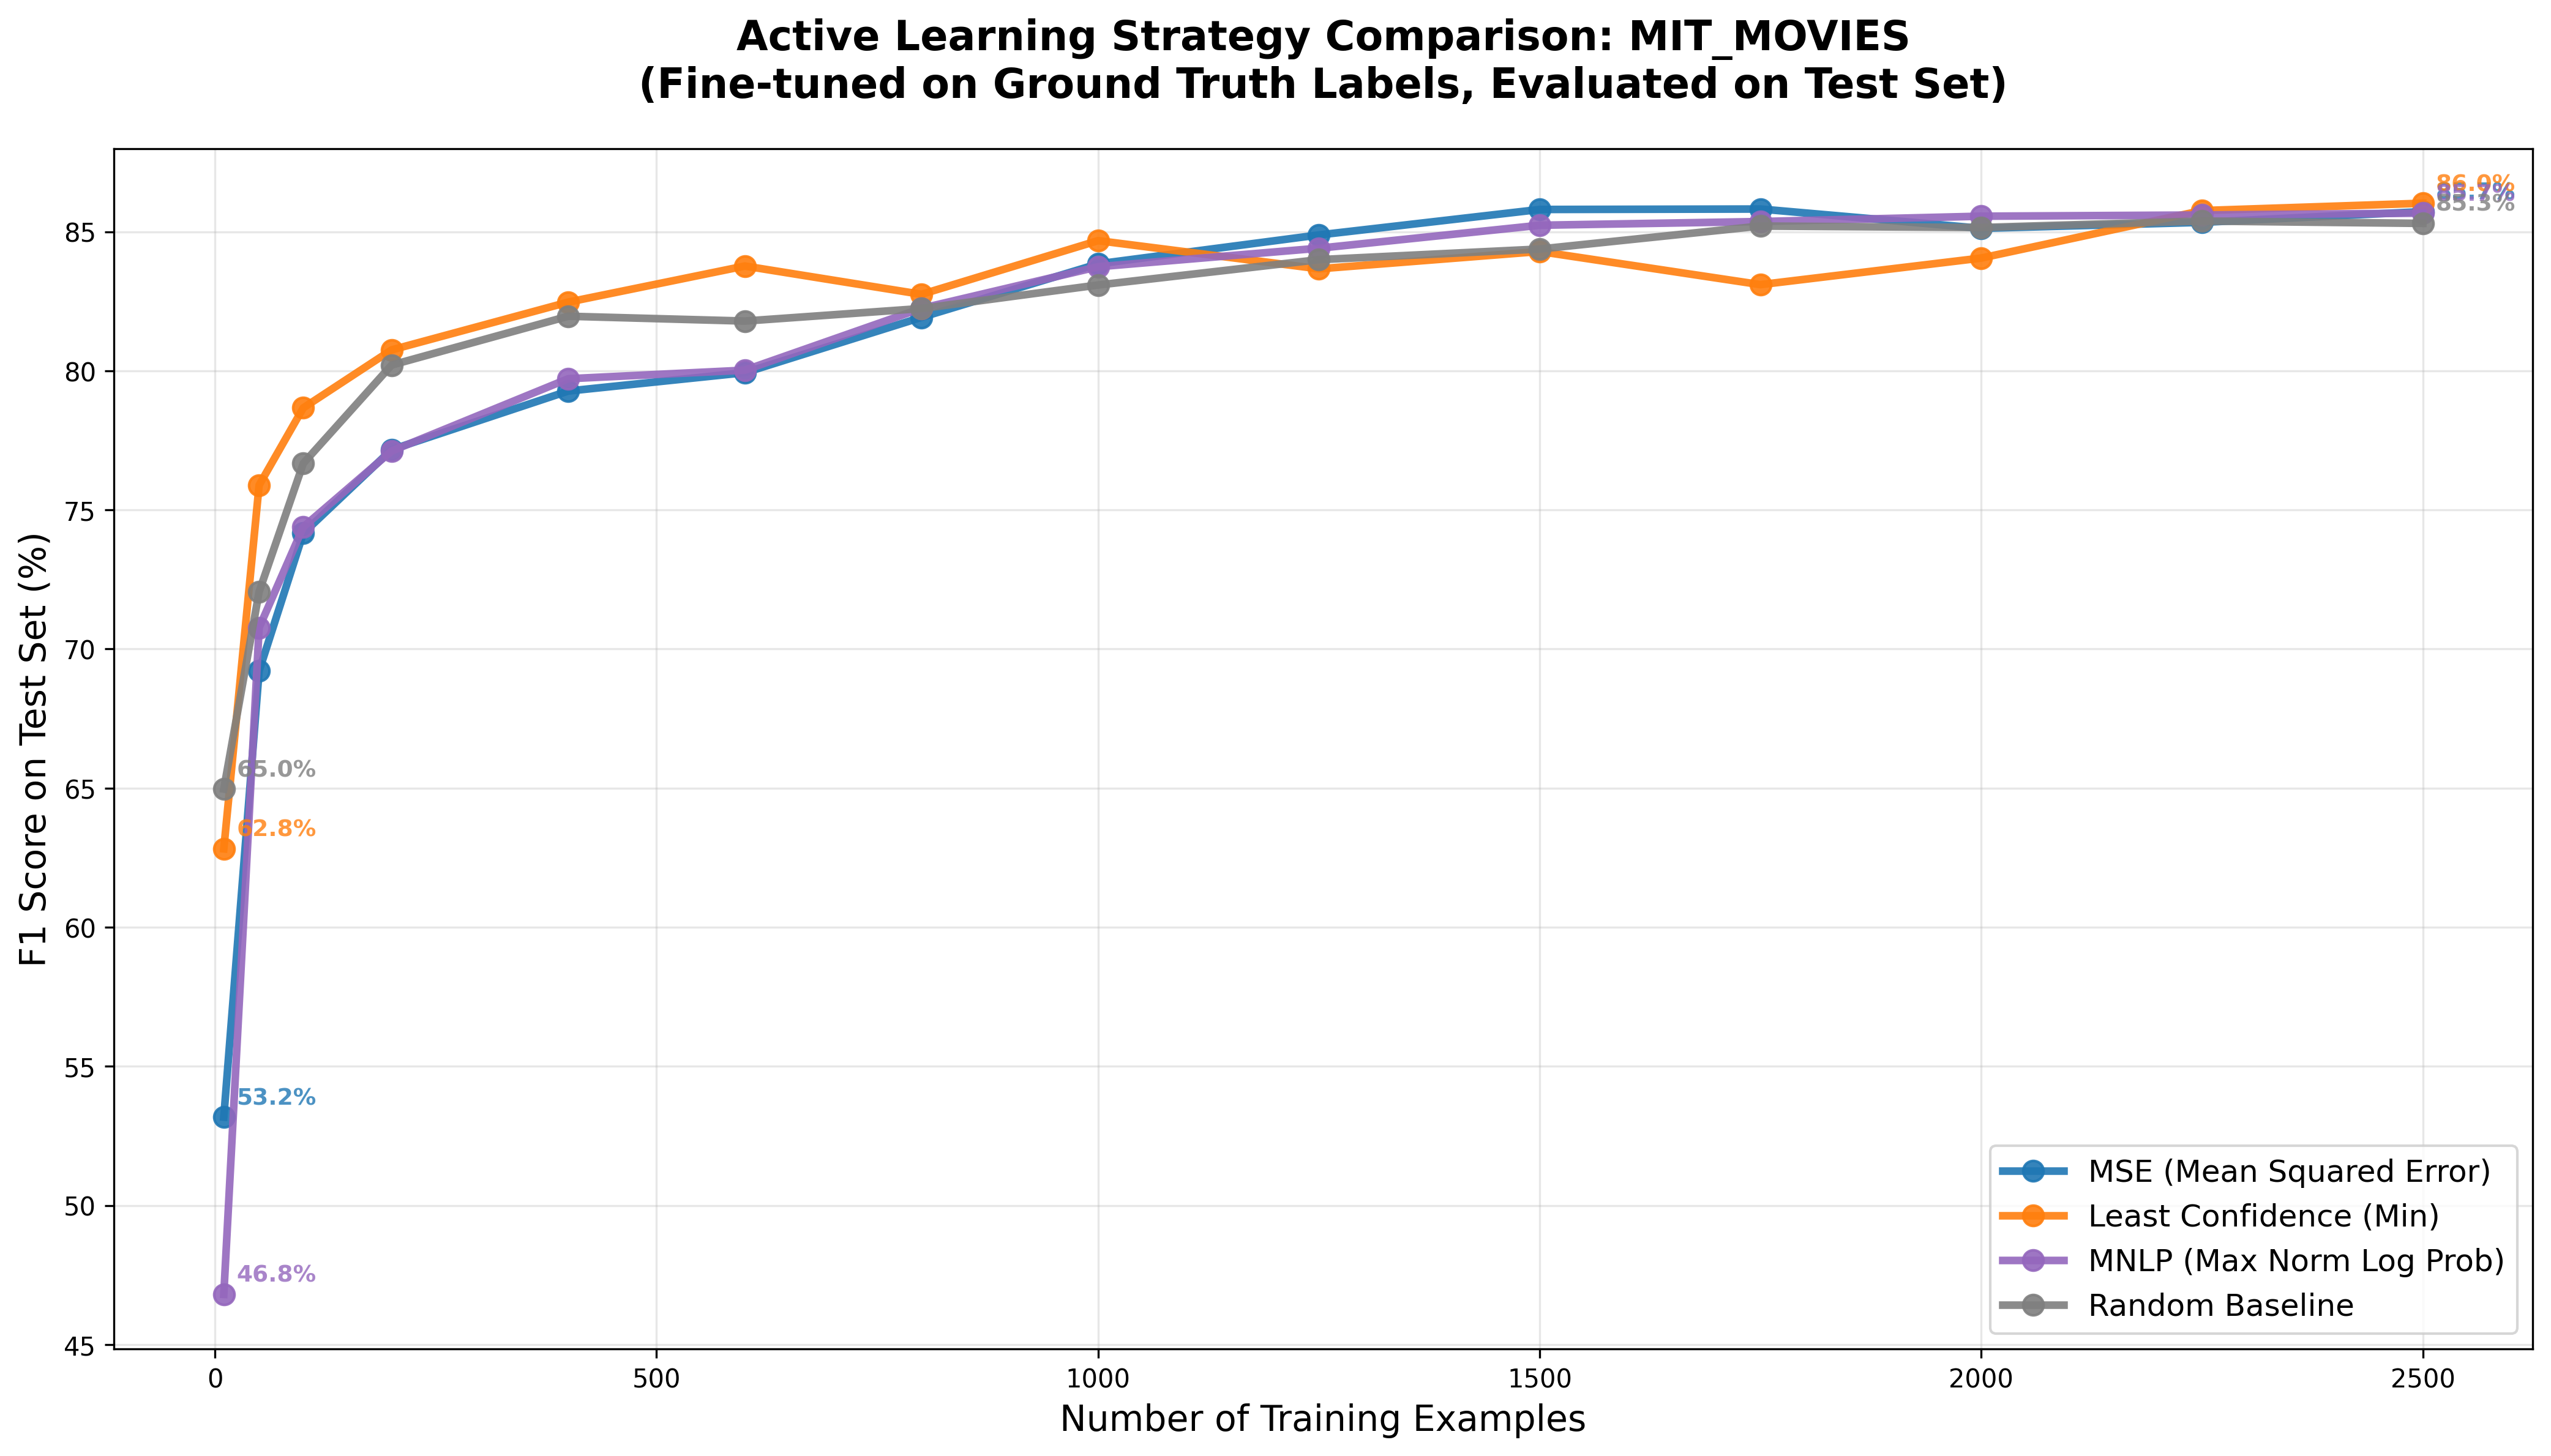
\includegraphics[width=0.78\textwidth]{figures/active_learning.png}
    \caption{Active learning strategy comparison on MIT Movies. Each line shows test set \fone{} as a function of the number of training examples selected by that strategy. All strategies are fine-tuned on ground truth labels with LoRA. The largest gains occur between 50 and 400 labeled sentences. Beyond 1{,}500 examples, strategies converge, with Least Confidence (orange) ending slightly ahead.}
    \label{fig:active_learning}
\end{figure*}

\begin{multicols}{2}

The effectiveness of minimum confidence is intuitive for span-based models. Because GLiNER produces per-span scores, the weakest span in a sentence directly identifies an entity the model struggles with. More complex aggregations (MSE, MNLP) average across spans, diluting the signal when a sentence contains both easy and hard entities.

\subsection{GLiNER vs. LLM on Hard Examples}

Figure~\ref{fig:baseline_confidence} compares the zero-shot performance of GLiNER and Gemma 3 12B on progressively larger subsets of the worst confidence examples. The LLM consistently outperforms the base GLiNER model on these difficult sentences, reaching 68.2\% \fone{} at 2{,}500 examples vs. 40.9\% for GLiNER Base. This gap motivates the use of LLM labels as supplementary supervision for the examples where GLiNER is weakest.

\end{multicols}

% Baseline confidence figure (full width)
\begin{figure*}[t]
    \centering
    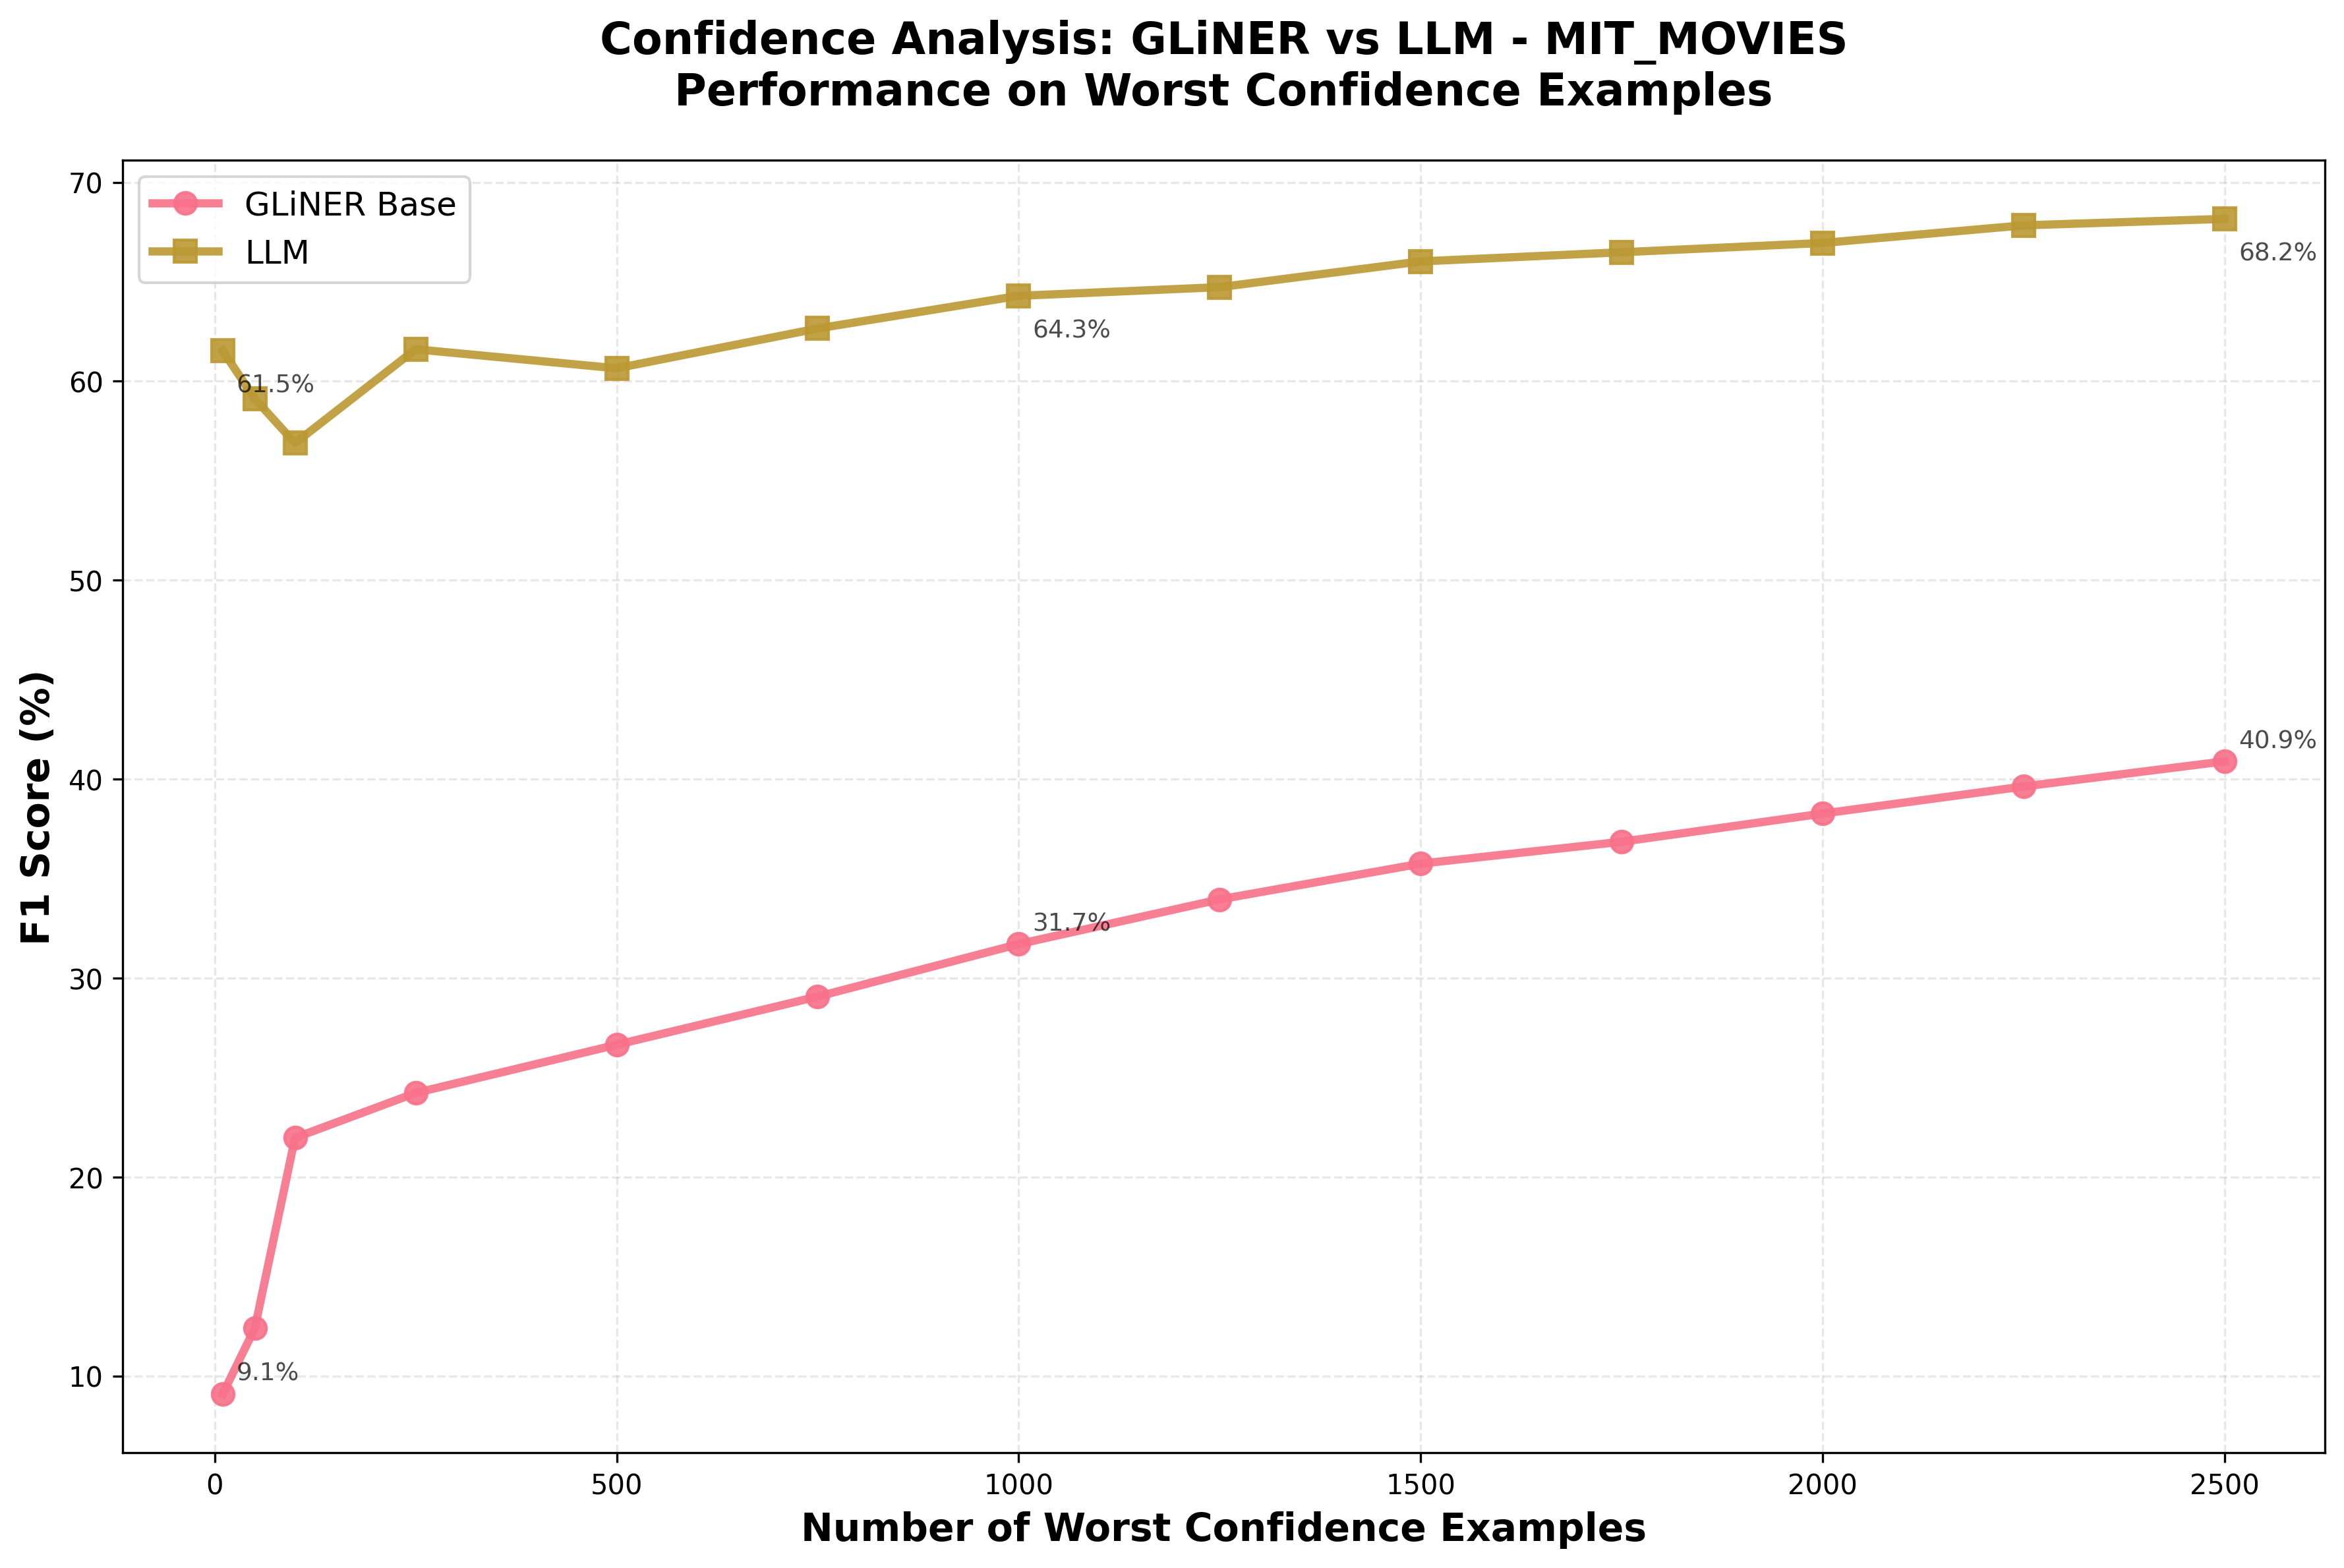
\includegraphics[width=0.75\textwidth]{figures/baseline_confidence.png}
    \caption{Zero-shot comparison between GLiNER Base and Gemma 3 12B on the worst confidence training examples (ranked by MSE). The LLM maintains a consistent advantage on examples where GLiNER is most uncertain, motivating the use of LLM labels as supplementary supervision for these difficult cases.}
    \label{fig:baseline_confidence}
\end{figure*}

\begin{multicols}{2}

\subsection{Ground Truth vs. LLM Labels}

Figure~\ref{fig:gt_vs_llm} shows what happens when GLiNER is fine-tuned on these hard examples using either human or LLM labels. Ground truth fine-tuning reaches 85.3 \fone{} at 2{,}500 examples. LLM label fine-tuning saturates around 69 \fone{}, close to the teacher's own accuracy. This confirms that synthetic labels inherit the teacher's performance ceiling.

\end{multicols}

% GT vs LLM figure (full width)
\begin{figure*}[t]
    \centering
    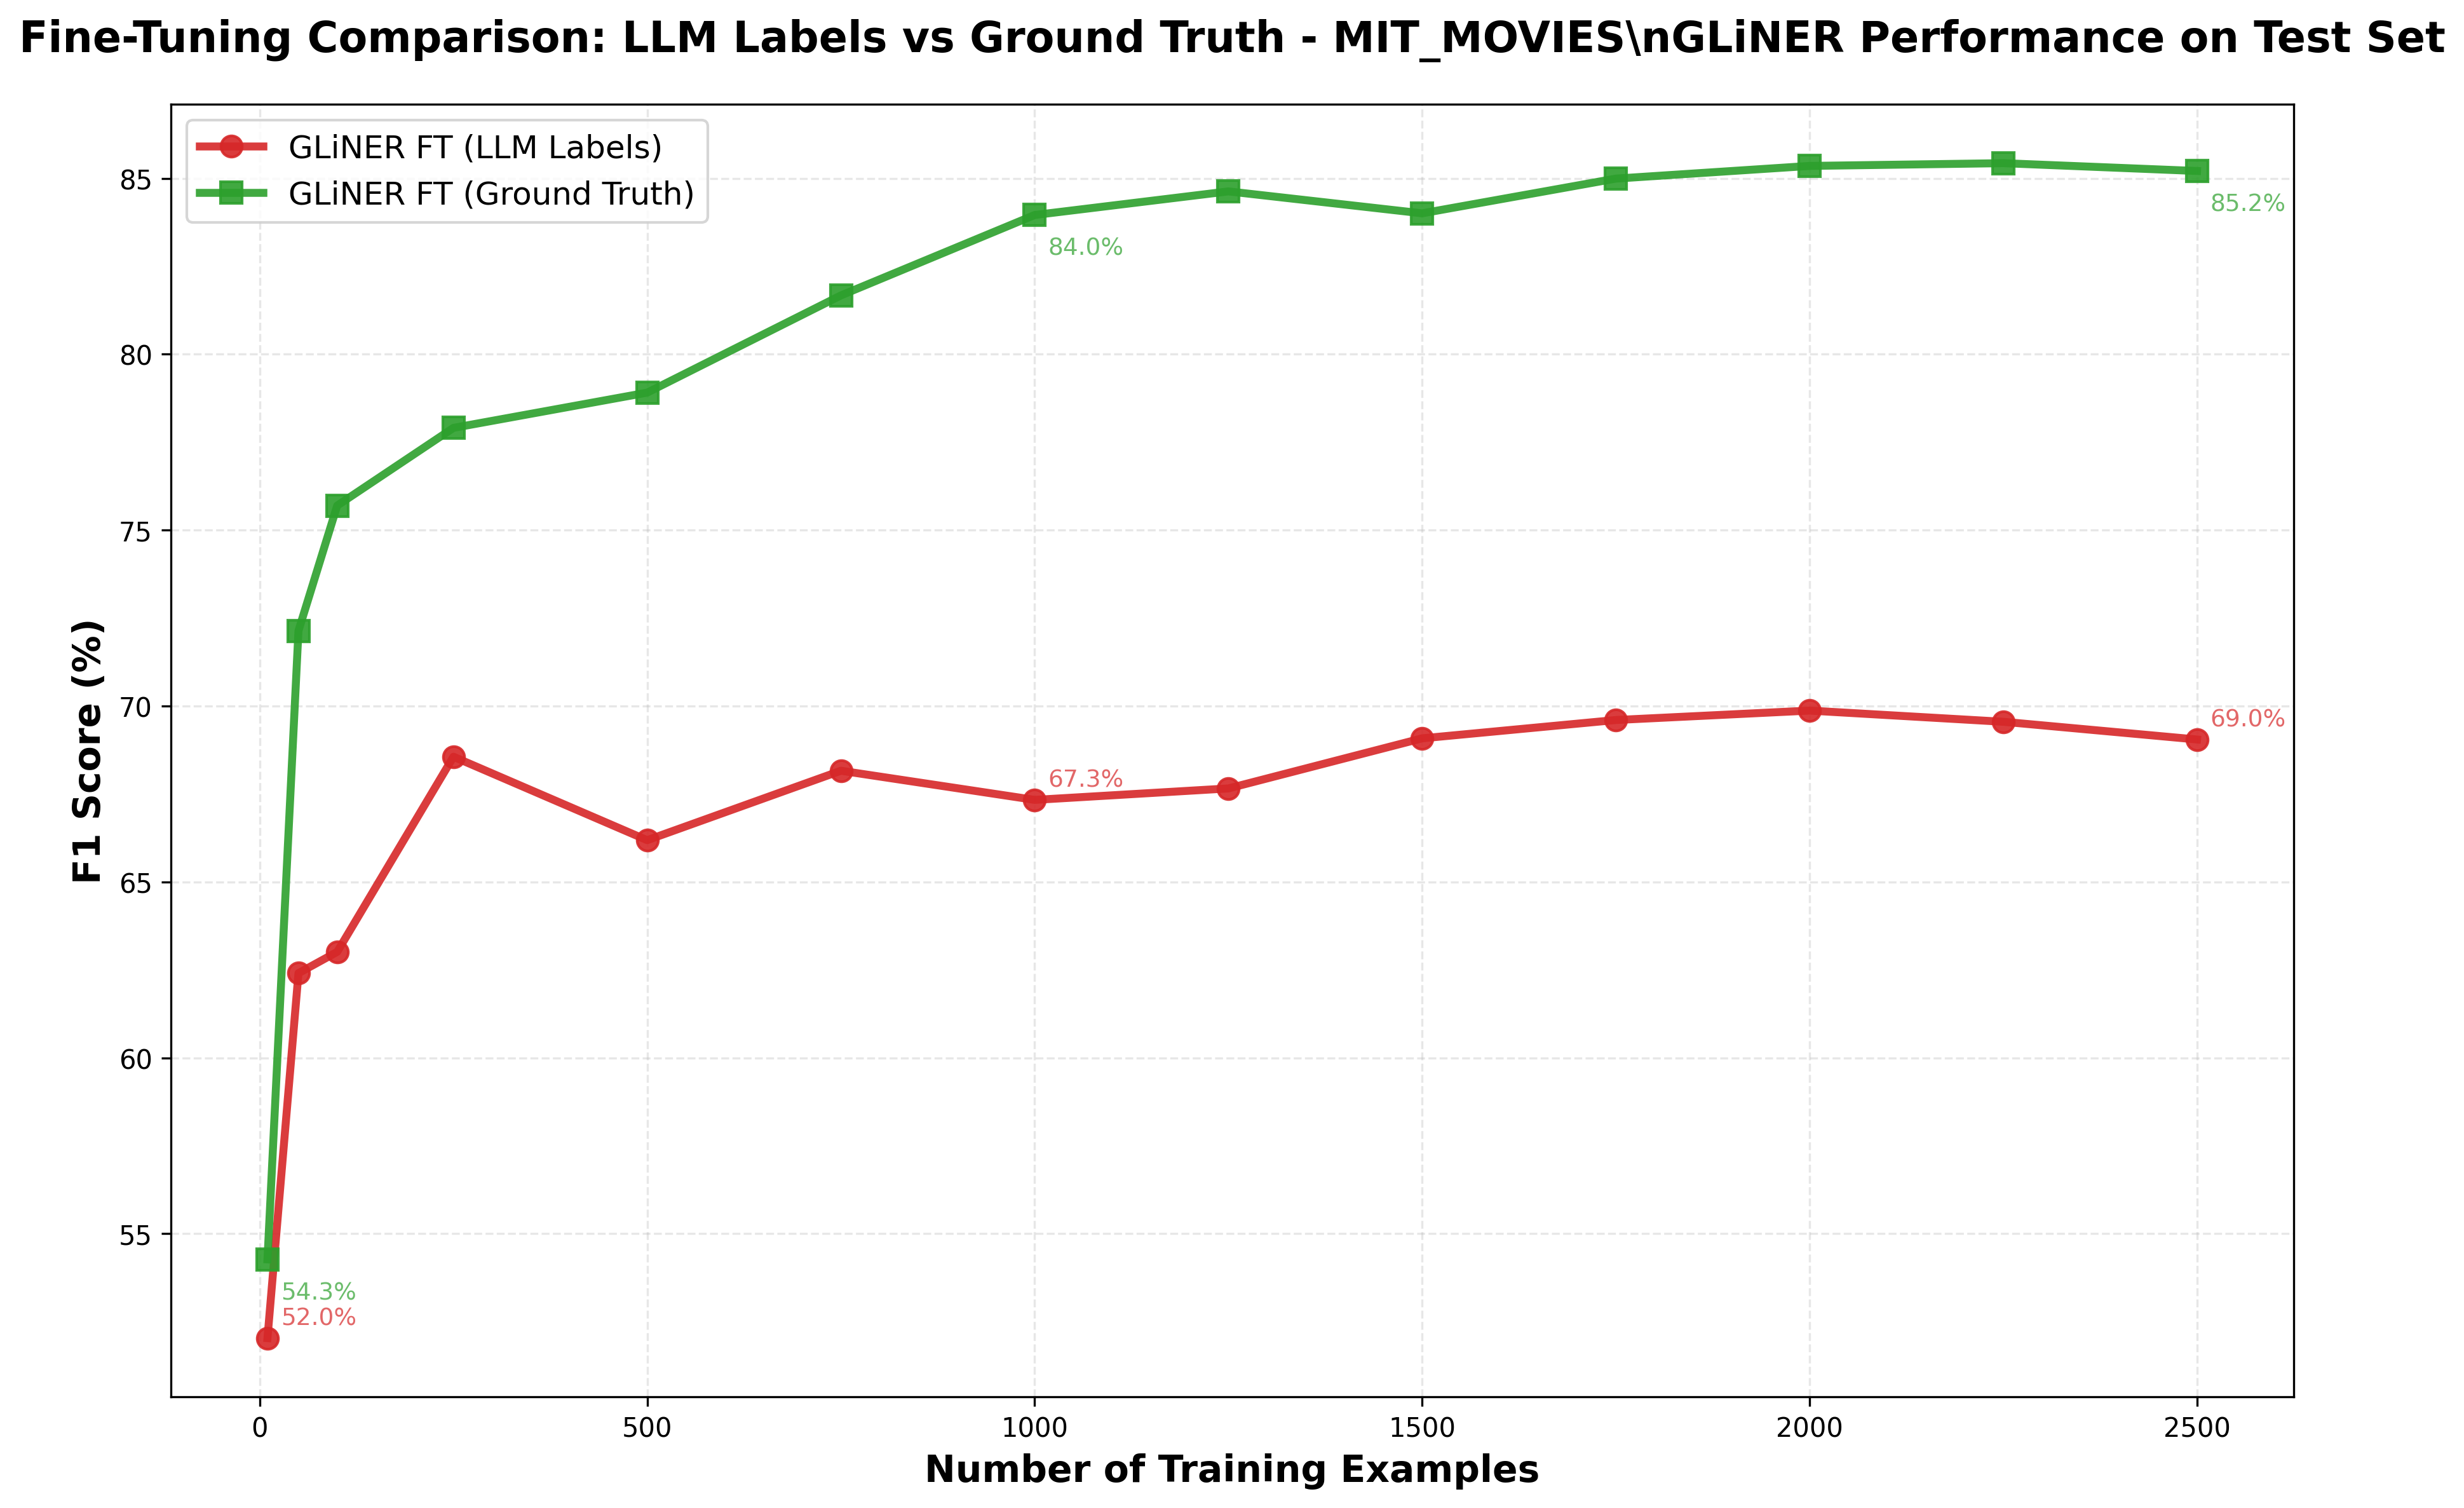
\includegraphics[width=0.75\textwidth]{figures/gt_vs_llm.png}
    \caption{Fine-tuning comparison: Ground truth labels (green) vs. Gemma 3 12B synthetic labels (red) on MSE-ranked worst confidence sentences, evaluated on the test set. Ground truth fine-tuning reaches 85.3\% \fone{}, while LLM labels saturate near the teacher's own performance (${\sim}$69\%). The gap confirms that synthetic labels alone cannot push the student beyond the teacher.}
    \label{fig:gt_vs_llm}
\end{figure*}

\begin{multicols}{2}

\subsection{Mixed Supervision Results}

Figure~\ref{fig:mixed} and Table~\ref{tab:mixing} present the central finding: mixing human and synthetic labels. With 1{,}000 examples and a 75/25 human/synthetic split, the model reaches 84.1 \fone{}, within one point of full supervision. A 50/50 split still achieves above 80 \fone{} at moderate budgets. Pure synthetic training (0\% GT) saturates around 70 \fone{}.

\end{multicols}

% Mixed figure (full width)
\begin{figure*}[t]
    \centering
    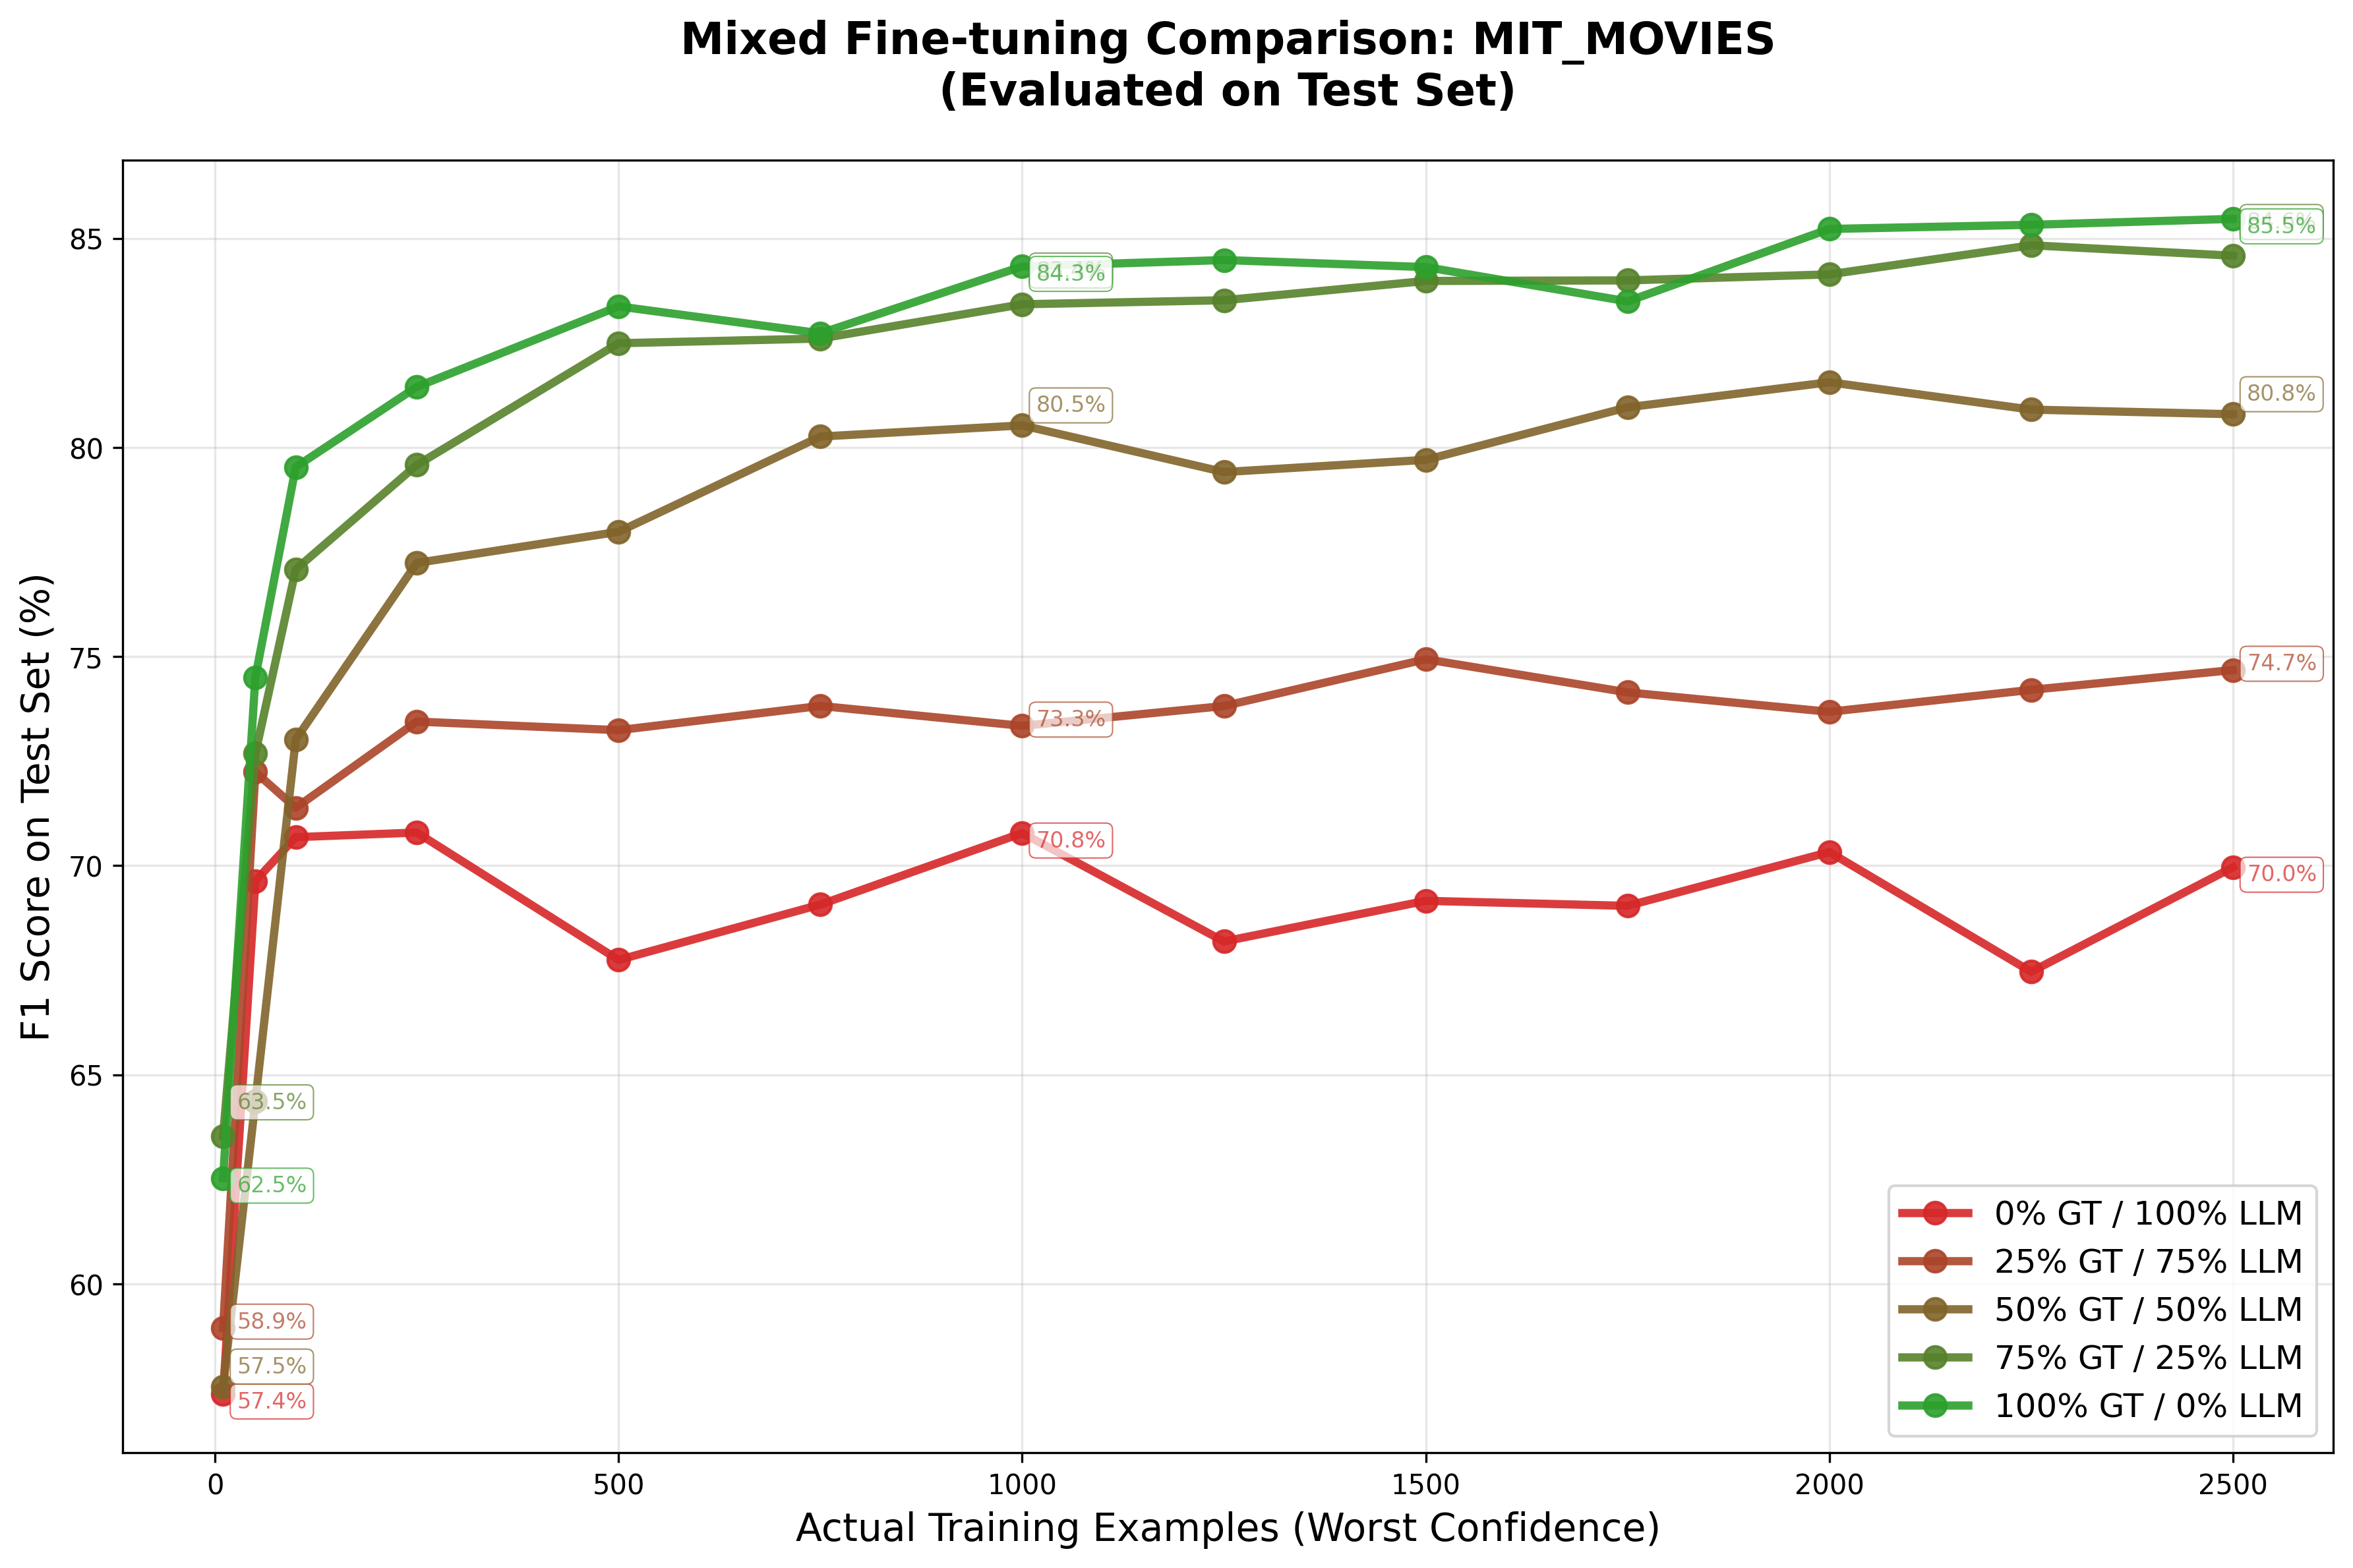
\includegraphics[width=0.78\textwidth]{figures/mixed_ft_min.png}
    \caption{Mixed fine-tuning results using minimum confidence ranking. Each line represents a different ratio of ground truth (GT) to Gemma 3 12B labels. The 75\% GT / 25\% LLM curve (dark green) closely tracks the fully supervised 100\% GT curve (bright green), while the pure LLM curve (red, 0\% GT) saturates around 70\% \fone{}. This demonstrates that a modest amount of synthetic labels can supplement human annotation with minimal performance loss.}
    \label{fig:mixed}
\end{figure*}

% Mixing table (full width, colored)
\begin{table}[H]
    \centering
    \small
    \begin{tabular}{r c c c c c}
        \toprule
        \rowcolor{headerblue!15}
        & \multicolumn{5}{c}{\textbf{Percentage of Ground Truth Labels}} \\
        \rowcolor{headerblue!15}
        \textbf{N} & \textbf{0\%} & \textbf{25\%} & \textbf{50\%} & \textbf{75\%} & \textbf{100\%} \\
        \midrule
        200 & \cellcolor{lightred!40}58.9 & 68.3 & 76.5 & \cellcolor{lightgreen!60}78.5 & \cellcolor{lightgreen}80.5 \\
        500 & \cellcolor{lightred!40}67.3 & 73.5 & 80.5 & \cellcolor{lightgreen}\textbf{84.1} & \cellcolor{lightgreen}84.0 \\
        1000 & \cellcolor{lightred!40}69.0 & 74.7 & 81.0 & \cellcolor{lightgreen!60}84.1 & \cellcolor{lightgreen}\textbf{85.3} \\
        1500 & \cellcolor{lightred!40}70.0 & 74.7 & 82.0 & \cellcolor{lightgreen!60}84.7 & \cellcolor{lightgreen}\textbf{85.5} \\
        2500 & \cellcolor{lightred!40}70.0 & 74.7 & 80.8 & \cellcolor{lightgreen}\textbf{85.5} & \cellcolor{lightgreen}85.5 \\
        \bottomrule
    \end{tabular}
    \caption{Test set \fone{} at different mixing ratios (minimum confidence ranking). Column headers show percentage of sentences with human labels; the rest use Gemma 3 12B labels. \colorbox{lightgreen}{Green} = near or at best performance. \colorbox{lightred!40}{Red} = pure synthetic labels. At 75\% GT, performance matches full supervision within 1 \fone{} point.}
    \label{tab:mixing}
\end{table}

\begin{multicols}{2}

\subsection{Cost Analysis}

Table~\ref{tab:cost} compares annual costs for processing one million NER tasks. Even the cheapest LLM (DeepSeek at 368 EUR/year) is nearly 100x more expensive than GLiNER's retraining cost (4 EUR/year). For applications where 85\% \fone{} is sufficient, GLiNER provides an economically compelling alternative with zero per-inference cost.

\end{multicols}

\begin{table}[H]
    \centering
    \small
    \begin{tabular}{l r c}
        \toprule
        \rowcolor{headerblue!15}
        \textbf{System} & \textbf{Annual Cost} & \textbf{Est. \fone{}} \\
        \midrule
        GPT-4o & 11{,}364 EUR & ${\sim}$98\% \\
        Claude Haiku 4.5 & 5{,}455 EUR & ${\sim}$94\% \\
        GPT-4o mini & 682 EUR & ${\sim}$95\% \\
        Gemini 2.5 Flash & 455 EUR & ${\sim}$93\% \\
        DeepSeek Chat & 368 EUR & ${\sim}$94\% \\
        \midrule
        \rowcolor{lightgreen!50}
        \textbf{GLiNER + LoRA (ours)} & \textbf{4 EUR} & \textbf{85\%} \\
        \bottomrule
    \end{tabular}
    \caption{Estimated annual cost for 1M NER tasks. LLM costs assume 1{,}000 input + 1{,}000 output tokens per task at published API prices. GLiNER cost = two retraining cycles per year on cloud GPU (${\sim}$2 EUR each) with zero inference cost.}
    \label{tab:cost}
\end{table}

% ============================================================
% 6. ANALYSIS
% ============================================================
\begin{multicols}{2}

\section{Analysis}

\paragraph{Why does minimum confidence work best?}
In sequence taggers, uncertainty is distributed across many BIO tokens, and aggregation through MNLP captures token-level ambiguity. In span-based models, each entity already carries a holistic confidence score. The minimum confidence of all spans directly identifies whether the sentence contains an entity the model finds difficult. More complex aggregations (MSE, MNLP) average across spans, diluting the signal from a single hard entity among several easy ones.

\paragraph{When do synthetic labels help vs. hurt?}
At a 75/25 human/synthetic split, synthetic labels provide additional training signal grounded by the human labels. When the ratio tips toward majority synthetic (25/75 or 0/100), the model learns the teacher's systematic errors (missing rare types, inconsistent boundaries), limiting performance.

\paragraph{Per-entity-type gains.}
The largest improvements from LoRA fine-tuning occur where the zero-shot model is weakest. Average ratings improves from 0.00 to 0.83 \fone{}, review from 0.09 to 0.22, character from 0.34 to 0.58. Common types (actor: 0.81 to 0.91, director: 0.76 to 0.89) also improve from higher baselines.

% ============================================================
% 7. LIMITATIONS
% ============================================================
\section{Limitations}

\paragraph{Single dataset.} All experiments use only MIT Movies, a slot-filling benchmark with clean annotations. Results may differ on noisier (WNUT) or more diverse (OntoNotes) datasets, or those with nested entities.

\paragraph{Simulated active learning.} Our single-round ranking does not include iterative re-ranking after each training round. True active learning would likely improve data efficiency further. Our results provide a lower bound.

\paragraph{Teacher quality.} Gemma 3 12B achieves only 69.7 \fone{} as annotator. A stronger teacher (GPT-4, larger Qwen) would likely produce better synthetic labels, potentially shifting the optimal mixing ratio.

\paragraph{No variance reporting.} Results are from single runs. LoRA fine-tuning can vary 1 to 3 \fone{} points across seeds. Some strategy differences may not be significant.

\paragraph{Missing baselines.} We do not compare against fine-tuned BERT or RoBERTa. Prior work reports BERT-base at ${\sim}$88.78 \fone{} on MIT Movies, which would contextualize our LoRA results.

% ============================================================
% 8. CONCLUSION
% ============================================================
\section{Conclusion}

We presented \method{}, a framework combining LoRA fine-tuning, uncertainty-based data selection, and strategic label mixing for efficient span-based NER. Three key findings emerge:

\textbf{First}, LoRA fine-tuning is sufficient for high quality NER adaptation, achieving 88.5 \fone{} while training only 4\% of parameters.

\textbf{Second}, simple minimum confidence outperforms more complex acquisition functions, reaching 80 \fone{} with just 200 labeled sentences (2\% of training data).

\textbf{Third}, a 75/25 human/synthetic label split performs within one \fone{} point of full supervision, offering a practical path to reducing annotation costs.

These results show that lightweight models with careful configuration can achieve strong NER performance at a fraction of the cost of LLM deployment, making production NER accessible to organizations with limited compute budgets.

\paragraph{Future Work.} We plan to validate on CoNLL 2003 and OntoNotes, implement iterative active learning with re-ranking, evaluate stronger teachers, and extend the approach to GLiNER-multitask for relation extraction.

\end{multicols}

% ============================================================
% REFERENCES
% ============================================================
\bibliographystyle{plainnat}
\bibliography{references}

\end{document}
